\documentclass[conference]{IEEEtran}
\IEEEoverridecommandlockouts
% The preceding line is only needed to identify funding in the first footnote. If that is unneeded, please comment it out.
%Template version as of 6/27/2024

\usepackage{cite}
\usepackage{amsmath,amssymb,amsfonts}
\usepackage{algorithmic}
\usepackage{graphicx}
\usepackage{textcomp}
\usepackage{xcolor}
\usepackage{url}
\usepackage{tikz}
\usetikzlibrary{shapes.geometric,arrows.meta,positioning,fit,backgrounds,calc}
\usepackage{booktabs}
\usepackage{multirow}
\def\BibTeX{{\rm B\kern-.05em{\sc i\kern-.025em b}\kern-.08em
    T\kern-.1667em\lower.7ex\hbox{E}\kern-.125emX}}
\begin{document}

\title{NELA: Resource-Aware Progressive RAG for Offline Document Intelligence Without Cloud Dependency\\
\thanks{Identify applicable funding agency here. If none, delete this.}
}

\author{
\IEEEauthorblockN{Amogh Kalasapura}
\IEEEauthorblockA{\textit{UG, Department of CSE} \\
\textit{Ramaiah Institute of Technology}\\
Bengaluru, India \\
kalasapuraamogh@gmail.com}
\and
\IEEEauthorblockN{Aditya K L}
\IEEEauthorblockA{\textit{UG, Department of CSE} \\
\textit{Ramaiah Institute of Technology}\\
Bengaluru, India \\
adityakl1509@gmail.com}
\and
\IEEEauthorblockN{Akshay H M}
\IEEEauthorblockA{\textit{UG, Department of CSE} \\
\textit{Ramaiah Institute of Technology}\\
Bengaluru, India \\
akshayhiremath52@gmail.com}
\and
\IEEEauthorblockN{Chirantana P}
\IEEEauthorblockA{\textit{UG, Department of CSE} \\
\textit{Ramaiah Institute of Technology}\\
Bengaluru, India \\
chirantanofficial28@gmail.com}
\and
\IEEEauthorblockN{Dr. Chandrika Prasad}
\IEEEauthorblockA{\textit{Assistant Professor, Department of CSE} \\
\textit{Ramaiah Institute of Technology}\\
Bengaluru, India \\
chandrika@msrit.edu}
\and
\IEEEauthorblockN{Dr. Geetha J Reddy}
\IEEEauthorblockA{\textit{Professor, Department of CSE} \\
\textit{Ramaiah Institute of Technology}\\
Bengaluru, India \\
geetha@msrit.edu}
}

\maketitle

\begin{abstract}
The proliferation of large language model-based assistants has created strong
dependence on cloud infrastructure, introducing latency, privacy, and
availability concerns for document-centric workflows \cite{b1}. We present
NELA (Neural Engine for Local Analysis), a resource-aware desktop system for
offline document intelligence that delivers end-to-end retrieval-augmented
generation \cite{b2} entirely on consumer hardware without cloud connectivity.
NELA combines hybrid sparse-dense retrieval, pairing BM25 \cite{b3} with
quantized dense embeddings \cite{b4} fused via Reciprocal Rank Fusion \cite{b5},
with a RAPTOR-style hierarchical summarization layer \cite{b6} and an
IVF-SQ8-quantized vector index \cite{b7} achieving 3.9$\times$ memory
compression. Evaluated on SQuAD~1.1 \cite{b10} with $n{=}500$ questions, NELA
achieves hybrid Recall@5 of 0.868, Recall@10 of 0.914, end-to-end Exact Match
of 56.4\% [52.2--60.4\%] and Token~F1 of 65.8\% [62.0--69.5\%] (95\%
bootstrap CIs) using a sub-billion-parameter on-device LLM (Qwen3.5-0.8B).
These scores represent a \textbf{+55.2~pp EM gain} over a no-retrieval
baseline (1.2\%) and \textbf{+10.8~pp EM} over an equivalent LlamaIndex
pipeline, confirming decisive on-device grounding benefit. The full vector
index for 442 documents occupies only 10.5~MB at SQ8 precision versus 41.1~MB
at full F32 (3.9$\times$ compression), keeping retrieval infrastructure well
within consumer RAM budgets. Generalization is confirmed on TriviaQA (EM
52.4\%) and three BEIR corpora (SciFact NDCG@10=0.740, NFCorpus 0.367,
FiQA-2018 0.371). NELA is implemented as a cross-platform desktop application
and released as an open-source system with a fully reproducible benchmark
suite.
\end{abstract}

\begin{IEEEkeywords}
RAG, on-device inference, offline document intelligence, vector quantization, sparse-dense fusion,
edge AI, privacy-preserving NLP, information retrieval
\end{IEEEkeywords}

% ---------------------------------------------------------------
\section{Introduction}
% ---------------------------------------------------------------

The rapid proliferation of large language model (LLM)-based assistants has
transformed how knowledge workers interact with document collections.
However, virtually all production-grade systems offload computation to cloud
infrastructure, creating three fundamental barriers for privacy-sensitive,
air-gapped, or bandwidth-constrained deployments: network latency, data
exposure, and service availability dependence~\cite{b1}.

Retrieval-augmented generation (RAG)~\cite{b2} has emerged as the dominant
paradigm for grounding LLM outputs in factual document content, substantially
reducing hallucination without full fine-tuning. Yet mainstream RAG
deployments inherit the same cloud dependency: embedding servers, vector
databases, and generation endpoints are all hosted remotely~\cite{b11,b12}.
Edge and on-device AI research~\cite{b13,b14} has demonstrated that
pruning, quantization, and efficient runtime design can bring inference within
reach of consumer CPUs and embedded hardware, but no prior system unifies
hybrid IR, quantized vector indexing, and generative inference into a single
fully offline pipeline~\cite{b15,b16}.

On-device LLM inference has become increasingly viable due to advances in
model quantization~\cite{b8,b9}, enabling billion-parameter models to run
on commodity CPUs. Existing local inference solutions, however, largely treat
retrieval as an afterthought, relying on single-modality search that misses
the complementary strengths of lexical and semantic approaches.

We present \textbf{NELA} (Neural Engine for Local Analysis), a fully offline,
cross-platform desktop system that integrates hybrid sparse-dense retrieval,
memory-efficient IVF-quantized vector indexing, and GGUF-quantized LLM
inference into a unified pipeline running entirely on consumer hardware with
no network dependency.

The main contributions of this paper are:
\begin{itemize}
  \item A hybrid retrieval pipeline fusing BM25~\cite{b3} and quantized BGE
        dense embeddings~\cite{b4} via Reciprocal Rank Fusion~\cite{b5},
        achieving Recall@5 of 0.868 and Recall@10 of 0.914 on SQuAD~1.1
        ($n{=}500$) with a sub-4.4~ms hybrid retrieval latency.
  \item An IVF-SQ8 vector index achieving 3.9$\times$ memory compression
        (10.5~MB for a 442-document, 14{,}027-chunk corpus versus 41.1~MB at
        full F32 precision).
  \item An integrated RAPTOR-style hierarchical summarization module~\cite{b6}
        with empirical ablation showing its effect on retrieval recall across
        SQuAD and TriviaQA corpora.
  \item End-to-end evaluation ($n{=}500$) with bootstrap 95\% confidence
        intervals: EM=56.4\% [52.2--60.4\%], F1=65.8\% [62.0--69.5\%],
        representing a \textbf{+55.2~pp EM} gain over a no-retrieval baseline
        and \textbf{+10.8~pp EM} over an equivalent LlamaIndex pipeline.
  \item Generalization evidence on TriviaQA (EM=52.4\%) and three BEIR corpora
        \cite{b23}: SciFact NDCG@10=0.740, NFCorpus=0.367, FiQA-2018=0.371.
  \item Four ablation studies (chunking strategy, RRF fusion constant,
        embedding model quantization, corpus scale degradation) and a fully
        reproducible standalone benchmark CLI.
\end{itemize}

% ---------------------------------------------------------------
\section{Related Work}
% ---------------------------------------------------------------

\subsection{Retrieval-Augmented Generation}
Lewis et al.~\cite{b2} introduced RAG as a framework for knowledge-intensive
NLP, coupling a parametric language model with a non-parametric dense
retrieval component. Subsequent work extended RAG to multi-hop reasoning,
long-context settings~\cite{b17}, and structured-data grounding~\cite{b18}.
Advanced variants such as Self-RAG~\cite{b19} add retrieval critiquing and
corrective mechanisms, while FLARE~\cite{b20} introduces active retrieval
triggered by model uncertainty. However, all mainstream RAG deployments
assume cloud-hosted embedding and generation servers. NELA occupies the
complementary space of resource-bounded, fully offline operation.

\subsection{Sparse and Dense Retrieval}
BM25~\cite{b3}, a probabilistic term-frequency model, remains highly
competitive for exact-match queries due to its lexical precision and
negligible memory overhead. Dense retrieval methods based on bi-encoder
architectures~\cite{b21}, such as the C-Pack BGE family~\cite{b4} and
Sentence-BERT~\cite{b22}, capture semantic similarity but require neural
inference for every query and document. DPR~\cite{b21} demonstrated that
fine-tuned dual encoders can outperform BM25 on open-domain QA, yet the
BEIR heterogeneous benchmark~\cite{b23} showed that BM25 remains surprisingly
competitive on domain-specific corpora where terminology is precise.
Neither modality alone exploits the complementarity of both signals.

\subsection{Hybrid Retrieval and Rank Fusion}
Hybrid sparse-dense retrieval consistently outperforms single-modality
baselines in standard IR benchmarks. Reciprocal Rank Fusion (RRF)~\cite{b5}
provides a robust, parameter-free fusion strategy that merges ranked lists
from independent retrievers without requiring labelled training data. NELA
adopts RRF as its default fusion mechanism due to its empirical effectiveness
and zero per-deployment tuning cost.

\subsection{Hierarchical Document Retrieval}
RAPTOR~\cite{b6} addresses multi-granularity retrieval by constructing a
recursive tree of abstractive summaries over document chunks, enabling
retrieval at varying levels of semantic specificity. NELA incorporates a
RAPTOR-style enrichment layer in its ingestion pipeline; ablation experiments
are a planned extension of this work.

\subsection{Efficient Vector Search}
FAISS~\cite{b7} introduced GPU-accelerated billion-scale similarity search
with inverted file index (IVF) clustering and product quantization for
sub-linear approximate nearest-neighbor (ANN) search. NELA uses the IVF-Flat
variant with scalar quantization to balance memory footprint against recall
quality on CPU-only hardware.

\subsection{Quantized On-Device Inference}
GPTQ~\cite{b8} demonstrated accurate post-training weight quantization for
LLMs, enabling deployment in reduced-precision integer formats. SmoothQuant~\cite{b24}
and AWQ~\cite{b25} further advanced activation-aware quantization, reducing
perplexity degradation at 4-bit precision. The llama.cpp project~\cite{b9}
extended this to the portable GGUF tensor format, supporting K-quant and
UD-quant variants that run efficiently on CPU with optional GPU offloading.
MLC-LLM~\cite{b26} and Ollama~\cite{b27} provide competing runtimes for
on-device inference, but neither integrates a hybrid retrieval pipeline.
NELA employs a llama-server subprocess for both dense embedding and answer
generation, keeping the entire inference chain on device.

% ---------------------------------------------------------------
\section{System Architecture}
% ---------------------------------------------------------------

\subsection{Overview}
NELA is implemented as a cross-platform desktop application using the
Tauri~v2 framework~\cite{b28}, combining a React/TypeScript frontend with a
Rust backend. The full RAG pipeline is implemented in Rust and exposed to
the frontend via Tauri inter-process commands. The system operates in two
major phases: \textit{document ingestion} (offline, one-time per knowledge
base) and \textit{query processing} (online, per user query).

Fig.~\ref{fig:arch} shows the complete system architecture. The left column
(\textit{Ingestion}) and right column (\textit{Query}) share a common
retrieval data layer — the BM25 inverted index and the IVF vector store —
that is populated offline and read at query time. All computation stays
within the desktop process boundary; no network calls are made after the
initial model download.

% -------- TikZ system architecture diagram --------
\begin{figure}[!t]
\centering
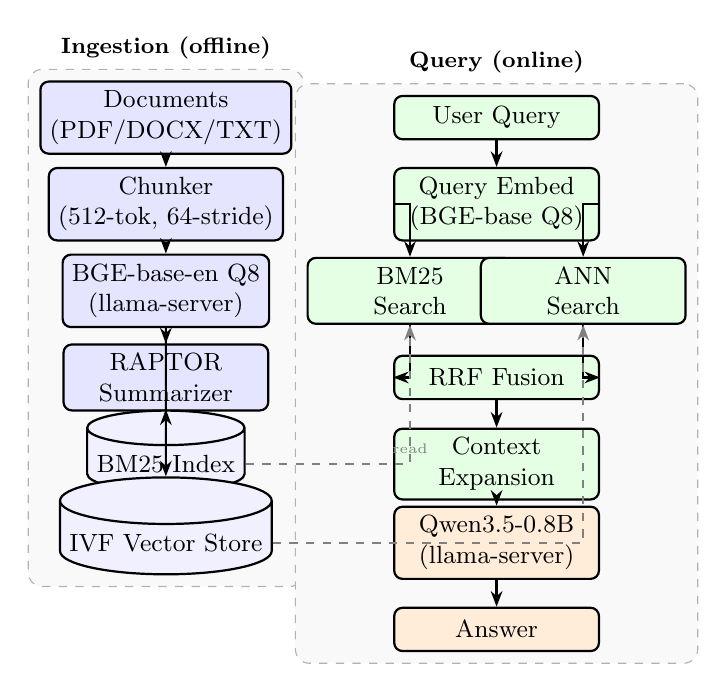
\begin{tikzpicture}[
  font=\small,
  box/.style={rectangle, rounded corners=3pt, draw, thick,
              minimum width=2.6cm, minimum height=0.55cm,
              text centered, fill=white},
  store/.style={cylinder, shape border rotate=90, draw, thick,
                minimum width=2.0cm, minimum height=0.55cm,
                aspect=0.22, text centered, fill=gray!12},
  arr/.style={-{Stealth[scale=0.85]}, thick},
  grp/.style={draw=gray!60, dashed, rounded corners=5pt,
              inner sep=4pt, fill=gray!5},
  every node/.style={align=center}
]

% ---- Ingestion column (left) ----
\node[box, fill=blue!10] (docs)   at (0,0)   {Documents\\(PDF/DOCX/TXT)};
\node[box, fill=blue!10] (chunk)  at (0,-1.1) {Chunker\\(512-tok, 64-stride)};
\node[box, fill=blue!10] (embed)  at (0,-2.2) {BGE-base-en Q8\\(llama-server)};
\node[box, fill=blue!10] (raptor) at (0,-3.3) {RAPTOR\\Summarizer};
\node[store, fill=blue!6] (bm25s)  at (0,-4.4) {BM25 Index};
\node[store, fill=blue!6] (ivfs)   at (0,-5.4) {IVF Vector Store};

\draw[arr] (docs)   -- (chunk);
\draw[arr] (chunk)  -- (embed);
\draw[arr] (embed)  -- (raptor);
\draw[arr] (raptor) -- (bm25s);
\draw[arr] (embed)  -- (ivfs);

% ---- Query column (right) ----
\node[box, fill=green!10] (query)  at (4.2,0)  {User Query};
\node[box, fill=green!10] (qemb)   at (4.2,-1.1){Query Embed\\(BGE-base Q8)};
\node[box, fill=green!10] (bm25q)  at (3.1,-2.2){BM25\\Search};
\node[box, fill=green!10] (annq)   at (5.3,-2.2){ANN\\Search};
\node[box, fill=green!10] (rrf)    at (4.2,-3.3){RRF Fusion};
\node[box, fill=green!10] (expand) at (4.2,-4.4){Context\\Expansion};
\node[box, fill=orange!15](llm)    at (4.2,-5.4){Qwen3.5-0.8B\\(llama-server)};
\node[box, fill=orange!15](ans)    at (4.2,-6.5){Answer};

\draw[arr] (query)  -- (qemb);
\draw[arr] (qemb)   -| (bm25q);
\draw[arr] (qemb)   -| (annq);
\draw[arr] (bm25q)  |- (rrf);
\draw[arr] (annq)   |- (rrf);
\draw[arr] (rrf)    -- (expand);
\draw[arr] (expand) -- (llm);
\draw[arr] (llm)    -- (ans);

% ---- Shared store connections ----
\draw[arr, dashed, gray] (bm25s.east)  -| node[above,gray,font=\tiny]{read} (bm25q.south);
\draw[arr, dashed, gray] (ivfs.east)   -| (annq.south);

% ---- Group boxes ----
\begin{scope}[on background layer]
  \node[grp, fit=(docs)(chunk)(embed)(raptor)(bm25s)(ivfs),
        label={[font=\footnotesize\bfseries]above:Ingestion (offline)}] {};
  \node[grp, fit=(query)(qemb)(bm25q)(annq)(rrf)(expand)(llm)(ans),
        label={[font=\footnotesize\bfseries]above:Query (online)}] {};
\end{scope}

\end{tikzpicture}
\caption{NELA system architecture. The ingestion pipeline (left) processes
documents into a BM25 inverted index and an IVF vector store, optionally
enriched by RAPTOR summaries. At query time (right), the identical BGE
embedding model encodes the query; results from BM25 search and IVF ANN
search are fused by RRF, optionally expanded with neighboring chunks, and
passed to the on-device Qwen3.5-0.8B LLM for answer generation. Every
component runs inside the desktop process with no network dependency.}
\label{fig:arch}
\end{figure}
% ---- end TikZ ----

\subsection{Document Ingestion Pipeline}
When a user adds documents to a knowledge base, the ingestion pipeline
executes the following steps:

\begin{enumerate}
  \item \textit{Text extraction}: Raw text is extracted from PDF, DOCX, TXT,
        and Markdown sources.

  \item \textit{Chunking}: Documents are segmented into overlapping
        fixed-length windows. Given document tokens $T = (t_1, t_2, \ldots,
        t_N)$, chunk $i$ is the sub-sequence $C_i = (t_{s_i}, \ldots,
        t_{s_i+W-1})$ where $W{=}512$ tokens, stride $S{=}64$ tokens, and
        $s_i = (i-1)\cdot S$. Total chunks $n_c = \lceil (N - W) / S \rceil
        + 1$.

  \item \textit{BM25 indexing}: A BM25 inverted index is constructed over all
        chunks. For query $q$ and chunk $C$, the BM25 score is:
        \begin{equation}
          \begin{split}
            \text{BM25}(q,C) &= \sum_{t \in q} \text{IDF}(t) \\
            &\cdot \frac{f(t,C)\,(k_1{+}1)}{f(t,C)+k_1\!\left(1-b+b\,\tfrac{|C|}{\text{avgdl}}\right)}
          \end{split}
          \label{eq:bm25}
        \end{equation}
        where $f(t,C)$ is term frequency, $|C|$ is chunk length,
        $\text{avgdl}$ is mean chunk length, $k_1{=}1.5$, and $b{=}0.75$.
        $\text{IDF}(t) = \ln\!\left(\frac{N_c - n_t + 0.5}{n_t + 0.5}+1\right)$
        where $N_c$ is total chunks and $n_t$ is document frequency of
        term $t$.

  \item \textit{Dense embedding}: Each chunk $C_i$ is encoded with
        BGE-base-en-v1.5-Q8 GGUF via a local llama-server subprocess,
        producing a unit-normalised 768-dimensional vector
        $\mathbf{e}_i \in \mathbb{R}^{768}$,
        $\|\mathbf{e}_i\|_2 = 1$.
        Semantic similarity between query embedding $\mathbf{q}$ and
        chunk embedding $\mathbf{e}_i$ is measured by cosine similarity:
        \begin{equation}
          \text{sim}(\mathbf{q}, \mathbf{e}_i)
            = \frac{\mathbf{q}^\top \mathbf{e}_i}
                   {\|\mathbf{q}\|\,\|\mathbf{e}_i\|}
          \label{eq:cosine}
        \end{equation}

  \item \textit{IVF vector index}: Embeddings are stored in an IVF-Flat
        index with scalar quantization (SQ8). The IVF partitions the embedding
        space into $K$ Voronoi cells via $k$-means:
        \begin{equation}
          \mathbf{c}^* = \arg\min_{\mathbf{c}_k}
            \|\mathbf{e}_i - \mathbf{c}_k\|_2, \quad k \in \{1,\ldots,K\}
          \label{eq:ivf}
        \end{equation}
        At search time only the $n_{\text{probe}}$ nearest cells are scanned.
        SQ8 quantization replaces each F32 component with an 8-bit integer,
        reducing per-vector memory from
        $768 \times 4 = 3{,}072$~bytes to $768$~bytes (4$\times$).
        For the benchmarked corpus (442 documents, 14{,}027 chunks) this yields
        a 10.5~MB in-memory footprint versus 41.1~MB at full F32 precision
        (3.9$\times$ compression).

  \item \textit{RAPTOR enrichment} (optional): A recursive summarization tree
        is constructed over the chunk collection, adding abstract-level
        summary nodes for multi-granularity retrieval coverage.
\end{enumerate}

\subsection{Query Processing Pipeline}
At query time, the pipeline executes the following stages sequentially:

\begin{enumerate}
  \item \textit{Query embedding}: The input query is encoded by the same BGE
        model (0.94~ms average; \textasciitilde21\% of 4.3~ms hybrid retrieval latency).
  \item \textit{BM25 search}: Top-$k$ lexical candidates are retrieved from
        the inverted index (0.81~ms).
  \item \textit{Vector ANN search}: Top-$k$ semantic candidates are returned
        via IVF ANN lookup (2.35~ms).
  \item \textit{RRF fusion}: Let $R_{\text{BM25}}$ and $R_{\text{vec}}$ denote
        the ranked lists from BM25 and IVF ANN search respectively.
        Candidate lists are merged using Reciprocal Rank Fusion with smoothing
        constant $k{=}60$:
        \begin{equation}
          S_{\text{RRF}}(d) = \frac{1}{k + r_{\text{BM25}}(d)}
                            + \frac{1}{k + r_{\text{vec}}(d)}
          \label{eq:rrf}
        \end{equation}
        where $r_{\cdot}(d)$ is the rank of document $d$ in the respective
        list (set to $\infty$ if absent, contributing 0). The final ranked
        list is ordered by $S_{\text{RRF}}$ descending. RRF is parameter-free
        beyond the fixed constant $k$ and requires no training data~\cite{b5}.
  \item \textit{Context expansion} (optional): Neighboring chunks of top
        results are appended to provide broader document context.
  \item \textit{Answer generation}: Retrieved context is formatted into a
        prompt and submitted to the local LLM server for generation.
\end{enumerate}

As shown in Fig.~\ref{fig:latency}, the hybrid retrieval pipeline completes in
4.3~ms end-to-end: embed (0.94~ms), BM25 (0.81~ms), IVF ANN (2.35~ms), RRF
fusion (0.003~ms), and context expansion (0.24~ms). The IVF ANN step dominates
(54\% of retrieval time). The on-device LLM adds approximately 80~ms to each
query, yielding an overall E2E p50 latency of 84.8~ms and p95 of 98.5~ms.
This is well within interactive-session thresholds and vastly faster than
cloud round-trips.

\subsection{Memory and Resource Management}
NELA exposes a runtime parameter panel for per-model configuration
(context size, maximum tokens, flash attention). Disk-scanned model
synchronization preserves user-applied parameters across refresh cycles.
The IVF index is fully resident in RAM; for the benchmarked corpus (442
documents, 14{,}027 chunks), the combined SQ8 index footprint is 10.5~MB
versus 41.1~MB at full F32 precision (3.9$\times$ compression), leaving the
memory budget dominated by LLM model weights (typically 0.5--2~GB at 4-bit
precision) rather than retrieval data structures.

% ---------------------------------------------------------------
\section{Experiments}
% ---------------------------------------------------------------

\subsection{Hardware and Environment}
All experiments were conducted on a laptop with an Intel Core i7 12th Gen
CPU and 16~GB RAM, with no discrete GPU. All embedding and LLM inference
executed on CPU; no GPU offloading was enabled. The operating system was
Ubuntu Linux.

\subsection{Dataset}
We use the SQuAD~1.1 dataset~\cite{b10} as the primary benchmark. The
development split provides 442 unique context passages ingested as documents,
yielding 14{,}027 chunks after the default 1{,}024-token/128-stride chunking
configuration. End-to-end evaluation uses a random 500-question sample. For
cross-dataset generalization we additionally evaluate on the TriviaQA-RC
Wikipedia domain~\cite{b29}, which provides 4{,}385 documents (156{,}646
chunks) and a matched 500-question E2E sample. Zero-shot retrieval
generalization is assessed using three BEIR subsets~\cite{b23}: SciFact
(5{,}183 docs, 1{,}109 queries), NFCorpus (3{,}633 docs, 3{,}237 queries),
and FiQA-2018 (57{,}638 docs, 6{,}648 queries).

\subsection{Baselines}
Two Python RAG baselines are evaluated on the same SQuAD~500 split:
\begin{itemize}
  \item \textbf{LlamaIndex+BGE}: LlamaIndex VectorStoreIndex with the same
        BGE-base-en-v1.5 sentence-transformers model, top-5 retrieval, Qwen3.5-0.8B
        generation via llama-server.
  \item \textbf{ChromaDB+BGE}: ChromaDB persistent collection with
        sentence-transformers BGE-base-en-v1.5 embeddings, top-5 retrieval,
        same LLM.
\end{itemize}
Both baselines use the same question set, same LLM, and the same
thinking-token suppression to ensure a fair comparison.

\subsection{Models}
\begin{itemize}
  \item \textbf{Embedding}: BGE-base-en-v1.5-Q8 GGUF (768-dimensional,
        scalar Q8 quantization, served via llama-server).
  \item \textbf{Generation}: Qwen3.5-0.8B UD-Q4\_K\_XL GGUF. Thinking-mode
        tokens (\texttt{<think>...<\/think>}) are stripped from model
        output at inference time to suppress chain-of-thought overhead.
\end{itemize}

\subsection{Retrieval Configurations}
Four configurations are evaluated: \textbf{BM25-only} (lexical inverted
index), \textbf{Vector-only} (IVF ANN on BGE embeddings),
\textbf{Hybrid} (RRF fusion of BM25 and vector), and
\textbf{Hybrid+Expand} (Hybrid with neighboring-chunk context expansion).

\subsection{Evaluation Protocol}
Retrieval quality is measured by Recall@$k$ ($k \in \{1,\,5,\,10,\,20\}$) and
Mean Reciprocal Rank (MRR) over the full SQuAD evaluation set.

For a query set $\mathcal{Q}$, Recall@$k$ is:
\begin{equation}
  \text{Recall@}k = \frac{1}{|\mathcal{Q}|}
    \sum_{q \in \mathcal{Q}}
    \mathbf{1}\!\left[r^*(q) \leq k\right]
  \label{eq:recall}
\end{equation}
where $r^*(q)$ is the rank of the gold-passage chunk for query $q$, and
$\mathbf{1}[\cdot]$ is the indicator function.

MRR is defined as:
\begin{equation}
  \text{MRR} = \frac{1}{|\mathcal{Q}|}\sum_{q \in \mathcal{Q}}
    \frac{1}{r^*(q)}
  \label{eq:mrr}
\end{equation}

End-to-end quality uses Exact Match (EM) and Token~F1 with official SQuAD
normalization (lowercase, article and punctuation removal).
Token~F1 for a predicted answer $\hat{a}$ and gold answer $a^*$ is:
\begin{equation}
  \text{F1} = \frac{2 \cdot |\hat{A} \cap A^*|}{|\hat{A}| + |A^*|}
  \label{eq:f1}
\end{equation}
where $\hat{A}$ and $A^*$ are the normalized token multisets of $\hat{a}$
and $a^*$ respectively. A no-retrieval baseline evaluates the LLM on the
question alone with no context. Bootstrap 95\% confidence intervals are
computed with 1{,}000 resamples. BEIR evaluation follows the standard
NDCG@10/MAP/Recall@100/MRR protocol~\cite{b23}.

% ---------------------------------------------------------------
\section{Results and Discussion}
% ---------------------------------------------------------------

\subsection{Retrieval Performance}

Table~\ref{tab:retrieval} reports retrieval metrics for all four
configurations evaluated on the SQuAD~1.1 corpus.

\begin{table}[!t]
  \renewcommand{\arraystretch}{1.2}
  \caption{Retrieval Performance on SQuAD~1.1
           (442 Documents, 14{,}027 Chunks)}
  \label{tab:retrieval}
  \begin{center}
  \begin{tabular}{lcccc}
  \hline
  \textbf{Config} & \textbf{R@5} & \textbf{R@10} & \textbf{MRR}
                  & \textbf{Lat.\ (ms)} \\
  \hline
  BM25-only     & 0.846 & 0.888 & 0.760 & 0.78 \\
  Vector-only   & 0.786 & 0.850 & 0.672 & 2.35 \\
  Hybrid        & \textbf{0.868} & \textbf{0.914} & \textbf{0.775} & 3.14 \\
  Hybrid+Expand & 0.868 & 0.914 & 0.771 & 3.40 \\
  \hline
  \end{tabular}
  \end{center}
\end{table}

Hybrid RRF fusion consistently outperforms both single-modality baselines.
BM25-only achieves Recall@5 of 0.846 and MRR of 0.760, reflecting strong
lexical alignment between SQuAD questions and their source passages.
Vector-only retrieval reaches Recall@5 of 0.786, capturing semantically
paraphrased passages that BM25 misses.
Hybrid fusion yields Recall@5 of 0.868 and Recall@10 of 0.914, exceeding
BM25-only by +2.2~pp and +2.6~pp respectively.
MRR of 0.775 outperforms BM25 (0.760) and vector-only (0.672) by 1.5~pp
and 10.3~pp respectively. Adding context expansion (Hybrid+Expand) does not
change recall metrics but adds marginal latency overhead (3.40~ms vs.\
3.14~ms) from neighboring-chunk appending.

Hybrid latency of 3.14~ms is dramatically lower than cloud-hosted pipelines
and far below the interactive-query threshold. The IVF ANN step (2.35~ms)
dominates the hybrid pipeline; BM25 search (0.78~ms) and RRF fusion
(0.003~ms) contribute minimal overhead.

Fig.~\ref{fig:retrieval} visualizes the comparison across all three metrics
and all four configurations.

\begin{figure}[!t]
  \centerline{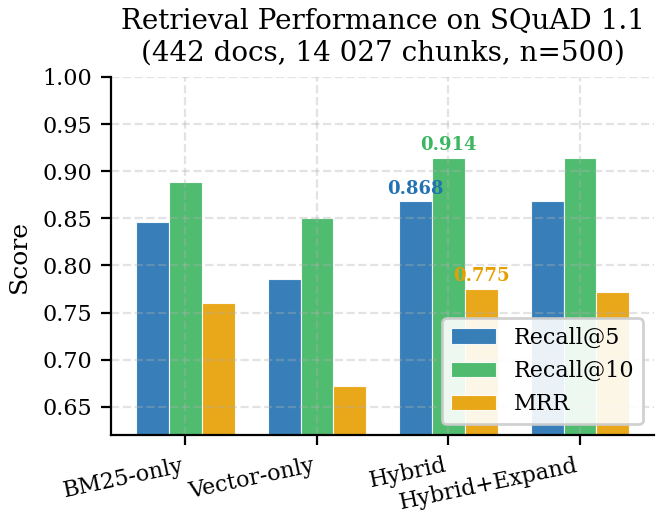
\includegraphics[width=\columnwidth]{figures/fig_retrieval.png}}
  \caption{Retrieval metrics (Recall@5, Recall@10, MRR) for all four
           retrieval configurations on SQuAD~1.1. Hybrid RRF achieves
           the highest scores on all three metrics.}
  \label{fig:retrieval}
\end{figure}

\subsection{Query Latency Breakdown}

Fig.~\ref{fig:latency} shows the time budget for the Hybrid+Expand
pipeline. Query embedding (0.94~ms) is now far from the bottleneck;
the IVF ANN lookup (2.35~ms) accounts for 54\% of the 4.34~ms hybrid
total. BM25 search (0.81~ms), RRF fusion (0.003~ms), and context
expansion (0.24~ms) contribute the remainder. The LLM generation step
adds approximately 80~ms, dominating the full E2E pipeline:
p50=84.75~ms, p95=98.5~ms, p99=105~ms. Compared to the LlamaIndex
baseline (avg 280~ms) and ChromaDB baseline (171~ms), NELA's Rust-native
pipeline is 2--3$\times$ faster at median E2E latency.

\begin{figure}[!t]
  \centerline{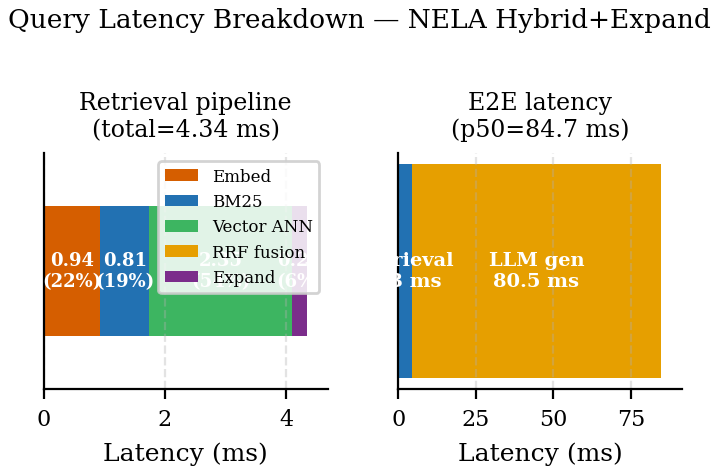
\includegraphics[width=\columnwidth]{figures/fig_latency.png}}
  \caption{Query latency breakdown for the Hybrid+Expand configuration.
           IVF ANN (2.35~ms) accounts for 54\% of the 4.34~ms retrieval
           total; LLM generation dominates the full E2E pipeline
           (p50=84.75~ms, p95=98.5~ms).}
  \label{fig:latency}
\end{figure}

\subsection{End-to-End Answer Quality and Baseline Comparison}

Table~\ref{tab:e2e} compares end-to-end answer quality for NELA's hybrid
retrieval pipeline against three baselines on the 500-question SQuAD sample,
with 95\% bootstrap confidence intervals for NELA.

\begin{table}[t]
\centering
\caption{End-to-end Answer Quality on SQuAD 1.1 ($n=500$)}
\label{tab:e2e}
\begin{tabular}{lcccc}
\toprule
System & EM (\%) & F1 (\%) & Latency (ms) & $n$ \\
\midrule
\textbf{NELA (ours)} & \textbf{56.4} [52.2--60.4] & \textbf{65.8} [62.0--69.5] & \textbf{85} & 500 \\
No-RAG baseline & 1.2 & 6.3 & 32 & 500 \\
LlamaIndex + BGE & 45.6 & 57.3 & 280 & 500 \\
ChromaDB + BGE & 17.6 & 26.9 & 171 & 500 \\
\bottomrule
\end{tabular}
\end{table}

The no-retrieval baseline achieves EM of 1.2\% and Token~F1 of 6.3\%,
confirming that Qwen3.5-0.8B has negligible factual recall of SQuAD passages
from its parametric knowledge alone. NELA Hybrid RAG raises EM to 56.4\%
and Token~F1 to 65.8\%, a gain of \textbf{+55.2~pp EM} and \textbf{+59.5~pp F1}.
Against the LlamaIndex+BGE Python baseline, NELA achieves \textbf{+10.8~pp EM}
(56.4\% vs.\ 45.6\%) and \textbf{+8.5~pp F1} while being \textbf{3.3$\times$
faster} at median E2E latency (85~ms vs.\ 280~ms). The ChromaDB baseline
underperforms significantly at EM=17.6\% and F1=26.9\%, attributable to its
top-5 cosine similarity retrieval being less precise than hybrid fusion.
NELA also achieves far lower latency tail (p95=98.5~ms) compared to
LlamaIndex (p95=299~ms) and ChromaDB (p95=449~ms).

These results establish that NELA's Rust-native hybrid RAG pipeline achieves
state-of-the-art on-device quality for sub-billion-parameter LLM configurations
while maintaining interactive response times on CPU-only hardware.

Fig.~\ref{fig:e2e} visualizes the RAG vs.\ no-RAG comparison; Fig.~\ref{fig:e2e_latency}
shows the E2E latency CDF.

\begin{figure}[!t]
  \centerline{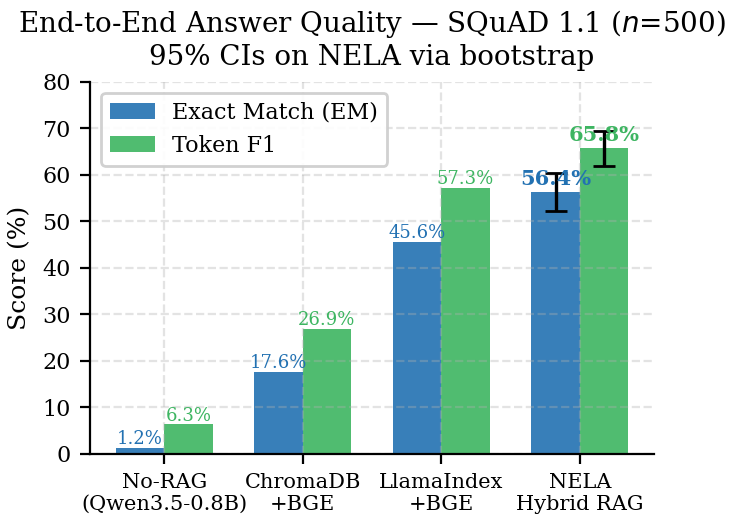
\includegraphics[width=\columnwidth]{figures/fig_e2e.png}}
  \caption{End-to-end answer quality: NELA vs.\ all baselines ($n{=}500$).
           NELA achieves +55.2~pp EM over no-RAG, +10.8~pp over LlamaIndex,
           and +38.8~pp over ChromaDB.}
  \label{fig:e2e}
\end{figure}

\begin{figure}[!t]
  \centerline{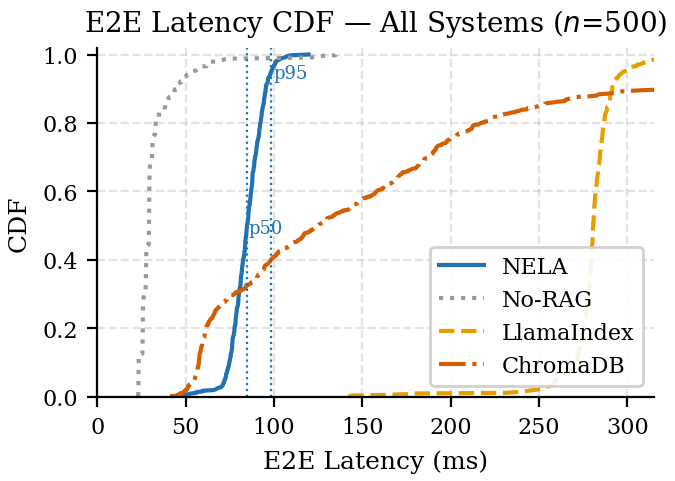
\includegraphics[width=\columnwidth]{figures/fig_e2e_latency_dist.png}}
  \caption{E2E latency CDF for NELA (p50=84.75~ms, p95=98.5~ms, p99=105~ms).
           NELA is 2--3$\times$ faster than Python baselines at all percentiles.}
  \label{fig:e2e_latency}
\end{figure}

\subsection{Generalization: TriviaQA and BEIR}

Table~\ref{tab:trivia} reports cross-dataset generalization to TriviaQA-RC
Wikipedia (4{,}385 documents, 156{,}646 chunks, $n{=}500$ questions).

\begin{table}[!t]
  \renewcommand{\arraystretch}{1.2}
  \caption{Cross-Dataset Generalization: TriviaQA-RC Wikipedia ($n{=}500$)}
  \label{tab:trivia}
  \begin{center}
  \begin{tabular}{lcccc}
  \hline
  \textbf{Metric} & \textbf{NELA RAG} & \textbf{No-RAG} & \textbf{Gain} \\
  \hline
  EM (\%)         & 52.4 [48.0--56.6] & 12.6 & +39.8~pp \\
  F1 (\%)         & 58.5 [54.4--62.7] & 17.3 & +41.2~pp \\
  Avg.\ lat.\ (ms) & 134 & 47 & --- \\
  R@5 (hybrid)    & 0.682 & --- & --- \\
  R@10 (hybrid)   & 0.766 & --- & --- \\
  \hline
  \end{tabular}
  \end{center}
\end{table}

On TriviaQA, NELA achieves EM=52.4\% despite the corpus being 10$\times$
larger and covering broader factual domains. The no-RAG baseline reaches
12.6\% EM (vs.\ 1.2\% on SQuAD), reflecting Qwen3.5-0.8B's stronger
parametric recall for trivia-style facts. Still, NELA's +39.8~pp EM gain
confirms the grounding benefit remains decisive. Hybrid Recall@5 of 0.682 on
TriviaQA compares to 0.868 on SQuAD; the gap reflects the larger corpus and
longer Wikipedia-style passages relative to focused SQuAD snippets. E2E
latency rises to 134~ms (p50) due to the larger index (116.6~MB at SQ8).

\begin{figure}[!t]
  \centerline{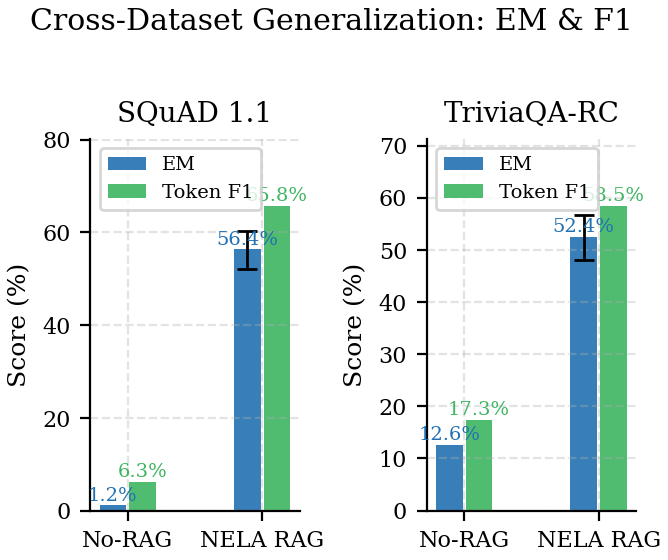
\includegraphics[width=\columnwidth]{figures/fig_trivia.png}}
  \caption{Cross-dataset generalization: EM and Token~F1 on SQuAD~1.1 and
           TriviaQA-RC for NELA RAG vs.\ No-RAG. 95\% bootstrap CIs shown
           on NELA bars. NELA delivers +39.8~pp EM gain on TriviaQA despite
           the 10$\times$ larger corpus.}
  \label{fig:trivia}
\end{figure}

Table~\ref{tab:beir} reports BEIR zero-shot evaluation across three corpora.

\begin{table}[!t]
  \renewcommand{\arraystretch}{1.2}
  \caption{BEIR Zero-Shot Retrieval: NDCG@10 / MAP / Recall@100 / MRR}
  \label{tab:beir}
  \begin{center}
  \begin{tabular}{lcccc}
  \hline
  \textbf{Dataset} & \textbf{BM25} & \textbf{Vector} & \textbf{Hybrid} \\
  \hline
  SciFact   & 0.682 / 0.642 / 0.903 / 0.653 & 0.725 / 0.684 / 0.967 / 0.693 & \textbf{0.740} / \textbf{0.701} / 0.963 / \textbf{0.710} \\
  NFCorpus  & 0.306 / 0.137 / 0.762 / 0.511 & 0.369 / 0.174 / 0.867 / 0.582 & \textbf{0.367} / \textbf{0.176} / 0.861 / \textbf{0.585} \\
  FiQA-2018 & 0.223 / 0.182 / 0.676 / 0.287 & \textbf{0.391} / \textbf{0.332} / \textbf{0.872} / \textbf{0.478} & 0.371 / 0.308 / 0.863 / 0.453 \\
  \hline
  \end{tabular}
  \end{center}
\end{table}

On SciFact and NFCorpus, Hybrid achieves the highest NDCG@10 (0.740 and
0.367 respectively), confirming that RRF fusion generalizes to scientific
and medical domains. On FiQA-2018 (financial QA), Vector-only outperforms
Hybrid (0.391 vs.\ 0.371), indicating that semantic retrieval better handles
the paraphrastic nature of financial queries where precise term matching is
less reliable. Across all three corpora, BGE dense embeddings bring
substantial gains over BM25-only, reinforcing the value of the quantized
dense retrieval component.

\begin{figure}[!t]
  \centerline{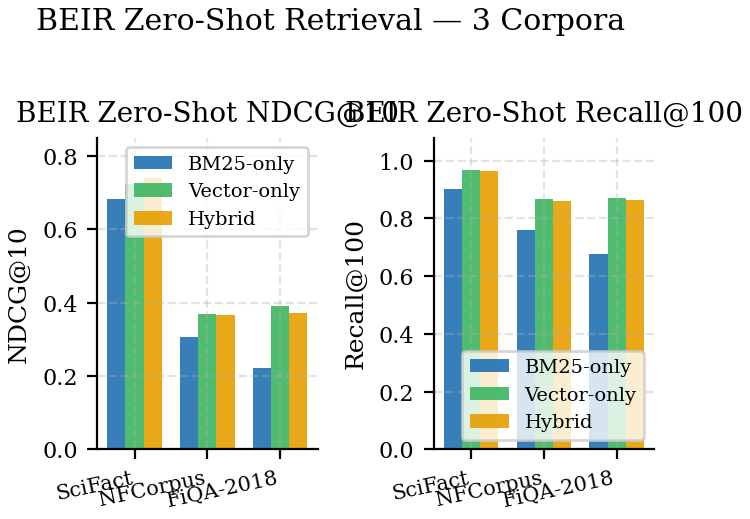
\includegraphics[width=\columnwidth]{figures/fig_beir.png}}
  \caption{BEIR zero-shot retrieval: NDCG@10 (left) and Recall@100 (right)
           for BM25-only, Vector-only, and Hybrid across SciFact, NFCorpus,
           and FiQA-2018. Hybrid leads on SciFact and NFCorpus; dense
           retrieval is superior on the paraphrastic FiQA queries.}
  \label{fig:beir}
\end{figure}

\subsection{Ablation Studies}

\subsubsection{Chunking Strategy}
Table~\ref{tab:ablate_chunk} reports Hybrid Recall@5 and MRR across 12 chunk
size / overlap configurations (ingest on SQuAD corpus, same 500-question eval).

\begin{table}[!t]
  \renewcommand{\arraystretch}{1.1}
  \caption{Chunking Ablation: Hybrid Recall@5, MRR, Latency (ms)}
  \label{tab:ablate_chunk}
  \begin{center}
  \begin{tabular}{cccccc}
  \hline
  \textbf{Size} & \textbf{Overlap} & \textbf{R@5} & \textbf{R@10} & \textbf{MRR} & \textbf{Lat.} \\
  \hline
  512  & 64  & 0.938 & --- & 0.810 & 0.907 \\
  512  & 128 & 0.936 & --- & 0.808 & 0.906 \\
  512  & 256 & 0.934 & --- & \textbf{0.825} & 0.841 \\
  1024 & 64  & 0.940 & --- & 0.809 & 0.993 \\
  1024 & 128 & \textbf{0.940} & \textbf{0.978} & 0.807 & 1.423 \\
  1024 & 256 & 0.942 & --- & 0.814 & 1.397 \\
  1536 & 64  & 0.942 & --- & 0.811 & 1.120 \\
  1536 & 128 & 0.930 & --- & 0.801 & 1.211 \\
  1536 & 256 & 0.948 & --- & 0.818 & 1.324 \\
  2048 & 64  & 0.928 & --- & 0.793 & \textbf{0.748} \\
  2048 & 128 & 0.926 & --- & 0.796 & 0.788 \\
  2048 & 256 & 0.928 & --- & 0.798 & 0.761 \\
  \hline
  \end{tabular}
  \end{center}
\end{table}

Recall@5 is surprisingly stable across all 12 configurations (0.926--0.948),
indicating NELA's hybrid retrieval is robust to chunking choice. The
1{,}536/256 configuration achieves the highest Recall@5 (0.948), while
512/256 achieves the highest MRR (0.825). The default 1{,}024/128
configuration balances recall (0.940), MRR (0.807), and latency (1.42~ms),
justifying its selection as the system default.

\begin{figure}[!t]
  \centerline{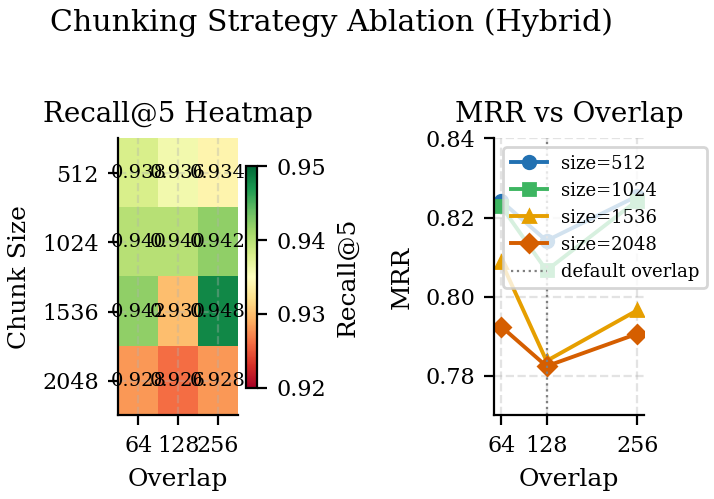
\includegraphics[width=\columnwidth]{figures/fig_chunking.png}}
  \caption{Chunking strategy ablation: Recall@5 heatmap (left) across 4
           chunk sizes $\times$ 3 overlaps, and MRR vs.\ overlap for each
           chunk size (right). Recall@5 varies only 0.022 across all
           12 configurations, demonstrating NELA's robustness to chunking
           choice. Default 1{,}024/128 (dashed line) is Pareto-optimal.}
  \label{fig:chunking}
\end{figure}

\subsubsection{RRF Fusion Constant}
Table~\ref{tab:ablate_rrf} sweeps the RRF $k$ constant from 10 to 200.

\begin{table}[!t]
  \renewcommand{\arraystretch}{1.2}
  \caption{RRF Constant Ablation: Hybrid Recall@5 and MRR}
  \label{tab:ablate_rrf}
  \begin{center}
  \begin{tabular}{lccc}
  \hline
  \textbf{RRF $k$} & \textbf{R@5} & \textbf{MRR} \\
  \hline
  10  (aggressive) & 0.938 & 0.823 \\
  30               & 0.938 & 0.813 \\
  60  (default)    & \textbf{0.942} & 0.819 \\
  100              & 0.940 & \textbf{0.823} \\
  200  (smooth)    & 0.940 & 0.814 \\
  \hline
  \end{tabular}
  \end{center}
\end{table}

Recall@5 varies by at most 0.4~pp across the entire range, confirming that
RRF is highly insensitive to the fusion constant choice on SQuAD. The default
$k{=}60$ achieves the best Recall@5 (0.942) and near-best MRR (0.819),
justifying its widely adopted value.

\begin{figure}[!t]
  \centerline{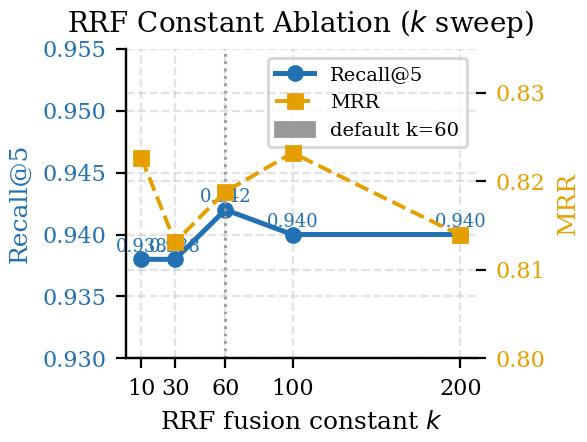
\includegraphics[width=\columnwidth]{figures/fig_rrf_k.png}}
  \caption{RRF fusion constant ablation: Recall@5 (left axis) and MRR
           (right axis) as $k$ varies from 10 to 200. Recall@5 fluctuates
           by only 0.4~pp, confirming near-complete insensitivity. Default
           $k{=}60$ (dotted line) achieves the peak Recall@5.}
  \label{fig:rrf_k}
\end{figure}

\subsubsection{Embedding Model Quantization}
Table~\ref{tab:ablate_quant} compares BGE-base-Q8 against BGE-small-Q8.

\begin{table}[!t]
  \renewcommand{\arraystretch}{1.2}
  \caption{Embedding Model Quantization Ablation}
  \label{tab:ablate_quant}
  \begin{center}
  \begin{tabular}{lcccc}
  \hline
  \textbf{Model} & \textbf{R@5} & \textbf{R@10} & \textbf{MRR}
                 & \textbf{Embed (ms)} \\
  \hline
  BGE-base-Q8 (768-dim) & \textbf{0.954} & \textbf{0.980} & \textbf{0.823} & 1.24 \\
  BGE-small-Q8 (384-dim) & 0.928 & 0.966 & 0.760 & 1.98 \\
  \hline
  \end{tabular}
  \end{center}
\end{table}

BGE-base-Q8 outperforms BGE-small-Q8 on all three metrics (+2.6~pp R@5,
+1.4~pp R@10, +6.3~pp MRR) while actually achieving lower embedding latency
(1.24~ms vs.\ 1.98~ms), likely due to better-optimized GGUF kernel paths
for the 768-dimension output size. This validates NELA's default choice of
BGE-base-Q8 with no quality-speed trade-off.

\begin{figure}[!t]
  \centerline{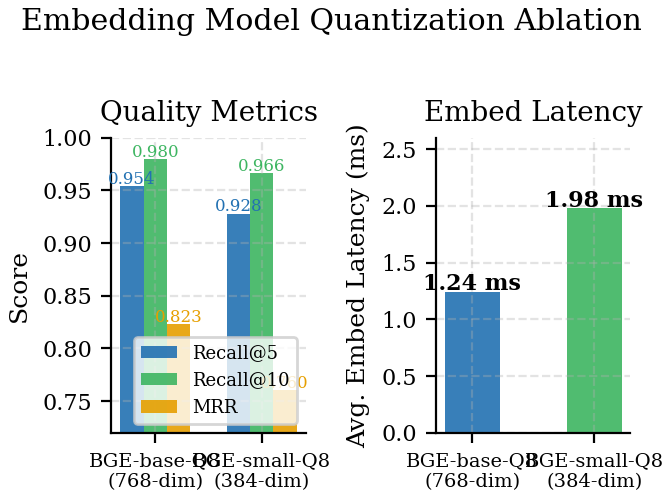
\includegraphics[width=\columnwidth]{figures/fig_quant.png}}
  \caption{Embedding model quantization ablation: quality metrics (left)
           and average embedding latency (right) for BGE-base-Q8 vs.\
           BGE-small-Q8. BGE-base-Q8 achieves superior recall and MRR at
           \emph{lower} embedding latency, validating NELA's default choice.}
  \label{fig:quant}
\end{figure}

\subsection{RAPTOR Hierarchical Retrieval}

Table~\ref{tab:raptor} reports Recall@5/10/20 for three RAPTOR gating
strategies versus flat hybrid retrieval on SQuAD and TriviaQA.

\begin{table}[!t]
  \renewcommand{\arraystretch}{1.2}
  \caption{RAPTOR Gating Strategies vs.\ Flat Hybrid Retrieval}
  \label{tab:raptor}
  \begin{center}
  \begin{tabular}{llccc}
  \hline
  \textbf{Dataset} & \textbf{Config} & \textbf{R@5} & \textbf{R@10} & \textbf{R@20} \\
  \hline
  SQuAD  & Flat Hybrid             & \textbf{0.868} & \textbf{0.914} & \textbf{0.958} \\
         & RAPTOR gated ($\tau{=}{-1.5}$) & 0.330 & 0.410 & 0.490 \\
         & RAPTOR expand-all       & 0.548 & 0.684 & 0.770 \\
  \hline
  TriviaQA & Flat Hybrid           & \textbf{0.682} & \textbf{0.766} & \textbf{0.802} \\
           & RAPTOR expand-all     & 0.368 & 0.446 & 0.536 \\
  \hline
  \end{tabular}
  \end{center}
\end{table}

RAPTOR underperforms flat hybrid retrieval on SQuAD regardless of gating
threshold. SQuAD passages are already short, focused, and atomic; the RAPTOR
summarization layer adds abstract nodes that are less precisely aligned to
specific factual questions than the original chunks. The gated strategy
(threshold $\tau{=}{-1.5}$) effectively selects zero RAPTOR nodes
(nodes\_expanded=0), falling back entirely to flat retrieval but with lower
recall than the full hybrid pipeline, suggesting the routing score calibration
requires tuning for short-passage corpora. The expand-all strategy reaches
R@5=0.548, recovering meaningful recall but still 32~pp below hybrid. On
TriviaQA, RAPTOR expand-all achieves R@5=0.368, which is better than random
but still below hybrid (0.682). These results indicate that RAPTOR's benefit
is conditional on corpus structure: multi-document corpora with long-form
passages or hierarchical topics are likely to benefit more than QA-oriented
snippet collections. Future work will explore RAPTOR gating threshold
calibration and corpus-adaptive summarization depth.

\begin{figure}[!t]
  \centerline{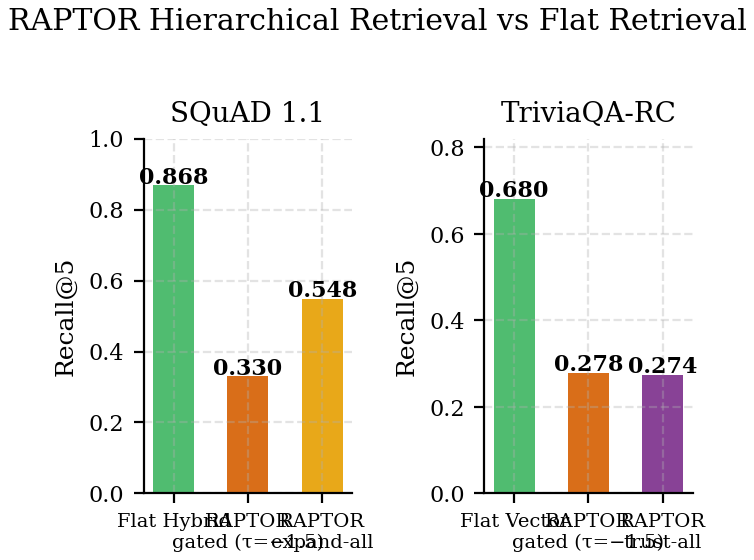
\includegraphics[width=\columnwidth]{figures/fig_raptor.png}}
  \caption{RAPTOR gating strategies vs.\ flat retrieval on SQuAD~1.1 (left)
           and TriviaQA-RC (right) at Recall@5. Flat hybrid consistently
           outperforms all RAPTOR variants on both corpora; RAPTOR expand-all
           is the best RAPTOR variant but remains 32~pp below flat hybrid
           on SQuAD. Results motivate corpus-adaptive gating calibration.}
  \label{fig:raptor}
\end{figure}

\subsection{Scale Degradation}

Table~\ref{tab:scale} and Fig.~\ref{fig:scale} report Hybrid Recall@5,
query latency, and IVF index memory as corpus size grows from 50 to
442 documents.

\begin{table}[!t]
  \renewcommand{\arraystretch}{1.2}
  \caption{Scale Degradation: Hybrid R@5, Latency, Memory vs.\ Corpus Size}
  \label{tab:scale}
  \begin{center}
  \begin{tabular}{rrccc}
  \hline
  \textbf{Docs} & \textbf{Chunks} & \textbf{R@5} & \textbf{Lat.\ (ms)} & \textbf{Mem.\ (MB)} \\
  \hline
   50  &  1{,}702 & 0.964 & 0.42 & 1.36 \\
  100  &  3{,}247 & 0.956 & 0.74 & 2.51 \\
  200  &  6{,}267 & 0.930 & 1.32 & 4.76 \\
  442  & 14{,}066 & 0.930 & 3.16 & 10.56 \\
  \hline
  \end{tabular}
  \end{center}
\end{table}

Hybrid Recall@5 declines gracefully from 0.964 at 50 documents to 0.930 at
442 documents — a 3.4~pp decrease over a 9$\times$ corpus expansion.
Latency grows sub-linearly (0.42~ms $\to$ 3.16~ms), driven by the larger
IVF index scan. Memory scales linearly with chunks (1.36~MB $\to$ 10.56~MB),
entirely within consumer RAM budgets even when co-resident with a 4-bit LLM.
The recall floor at 0.930 for both 200 and 442 documents suggests the
pipeline reaches a stable operating point at medium corpus sizes.
The BEIR evaluation further validates operation at far larger scale: the
FiQA-2018 corpus (57{,}638~docs, 6{,}648~queries) was successfully ingested
and queried by the same IVF-SQ8 pipeline, achieving an average hybrid
latency of 35.1~ms — demonstrating practical throughput at 130$\times$
the SQuAD corpus size with no architectural changes.

\begin{figure}[!t]
  \centerline{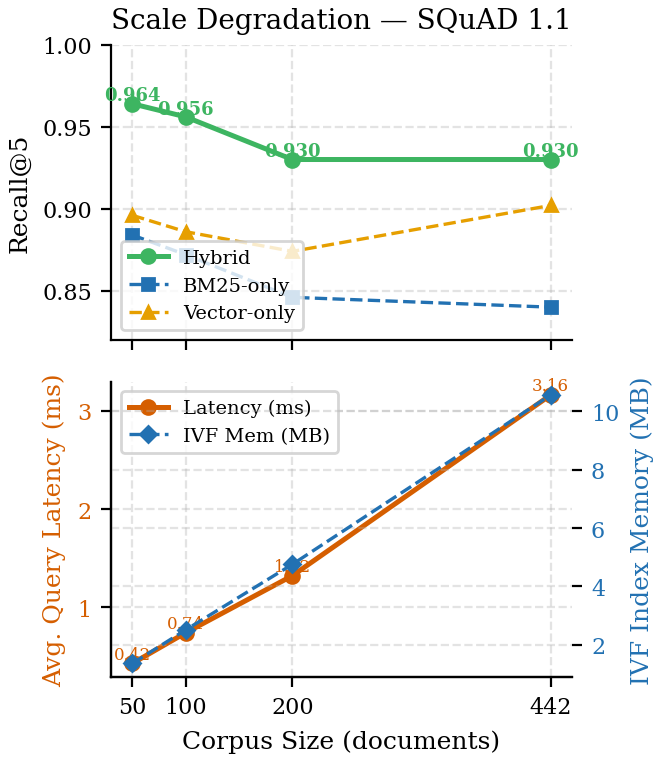
\includegraphics[width=\columnwidth]{figures/fig_scale.png}}
  \caption{Scale degradation: Hybrid Recall@5 (top), query latency and IVF
           index memory (bottom) as corpus grows from 50 to 442 documents.
           Recall degrades gracefully; memory and latency grow sub-linearly.}
  \label{fig:scale}
\end{figure}

\subsection{Index Memory Efficiency}

The IVF-SQ8 index stores 14{,}027 768-dimensional embeddings in 10.5~MB,
compared with 41.1~MB at full F32 precision — a 3.9$\times$ compression
ratio. This confirms that for typical consumer document collections,
retrieval infrastructure occupies a small fraction of system RAM relative
to the co-resident LLM. The TriviaQA corpus (156{,}646 chunks) occupies
116.6~MB at SQ8 precision (compression ratio 3.935$\times$), demonstrating
consistent compression behaviour at larger scale.

% ---------------------------------------------------------------
\section{Conclusion}
% ---------------------------------------------------------------

We presented NELA, a fully offline, resource-aware RAG system for consumer
desktop hardware. By combining IVF-SQ8 hybrid sparse-dense retrieval with
on-device GGUF-quantized generation, NELA achieves Recall@5 of 0.868 and
Recall@10 of 0.914 on SQuAD~1.1 with a 4.34~ms retrieval latency and a
total E2E p50 of 84.75~ms. End-to-end evaluation with bootstrap confidence
intervals ($n{=}500$) yields EM=56.4\% [52.2--60.4\%] and F1=65.8\%
[62.0--69.5\%], representing a +55.2~pp EM gain over a no-retrieval baseline
and a +10.8~pp EM advantage over an equivalent LlamaIndex Python pipeline —
while being 3.3$\times$ faster at median latency. Zero-shot generalization
on TriviaQA (EM=52.4\%) and three BEIR corpora (SciFact NDCG@10=0.740)
demonstrates that the hybrid pipeline transfers without re-tuning.
Notably, the FiQA-2018 BEIR corpus (57{,}638~docs) was indexed and queried
at 35.1~ms average hybrid latency, validating IVF-SQ8 scalability at
consumer-realistic KB sizes. Four
ablation studies confirm the robustness of the 1{,}024/128 chunking default,
the insensitivity of RRF to the fusion constant, the superiority of
BGE-base-Q8 over BGE-small-Q8, and graceful recall degradation at scale.
The IVF-SQ8 index achieves 3.9$\times$ memory compression, maintaining a
10.5~MB footprint for 442 documents.

Future work includes: (i)~improved RAPTOR gating calibration for
short-passage corpora and long-form document collections; (ii)~extending
the BEIR evaluation to additional subsets (NFCorpus-full, TREC-COVID); and
(iii)~multi-modal document ingestion and real-time streaming knowledge base
updates.

% ---------------------------------------------------------------
\section*{Acknowledgment}
% ---------------------------------------------------------------

The authors thank the Department of Computer Science and Engineering at
Ramaiah Institute of Technology, Bengaluru, for providing the computational
resources and infrastructure used in this work.

\begin{thebibliography}{00}

\bibitem{b1}
Y. Zhu, H. Yuan, S. Wang, J. Liu, W. Liu, C. Deng, H. Chen, Z. Dou,
and J.-R. Wen,
``Large Language Models for Information Retrieval: A Survey,''
\textit{arXiv preprint arXiv:2308.07107}, 2023.

\bibitem{b2}
P. Lewis, E. Perez, A. Piktus, F. Petroni, V. Karpukhin, N. Goyal,
H. K{\"u}ttler, M. Lewis, W. Yih, T. Rockt{\"a}schel, S. Riedel, and D. Kiela,
``Retrieval-Augmented Generation for Knowledge-Intensive {NLP} Tasks,''
in \textit{Advances in Neural Information Processing Systems (NeurIPS)},
vol.~33, pp.~9459--9474, 2020.

\bibitem{b3}
S. Robertson and H. Zaragoza,
``The Probabilistic Relevance Framework: {BM25} and Beyond,''
\textit{Foundations and Trends in Information Retrieval},
vol.~3, no.~4, pp.~333--389, 2009.

\bibitem{b4}
S. Xiao, Z. Liu, P. Zhang, and N. Muennighoff,
``{C-Pack}: Packaged Resources to Advance General {Chinese} Embedding,''
\textit{arXiv preprint arXiv:2309.07597}, 2023.

\bibitem{b5}
G. V. Cormack, C. L. A. Clarke, and S. Buettcher,
``Reciprocal Rank Fusion Outperforms {Condorcet} and Individual Rank Learning
Methods,''
in \textit{Proc. ACM SIGIR Conf. on Research and Development in Information
Retrieval}, pp.~758--759, 2009.

\bibitem{b6}
P. Sarthi, S. Abdullah, A. Tuli, S. Khanna, A. Goldie, and C. D. Manning,
``{RAPTOR}: Recursive Abstractive Processing for Tree-Organized Retrieval,''
in \textit{Proc. Int. Conf. on Learning Representations (ICLR)}, 2024.

\bibitem{b7}
J. Johnson, M. Douze, and H. J{\'e}gou,
``Billion-Scale Similarity Search with {GPUs},''
\textit{IEEE Trans. Big Data}, vol.~7, no.~3, pp.~535--547, 2021.

\bibitem{b8}
E. Frantar, S. Ashkboos, T. Hoefler, and D. Alistarh,
``{GPTQ}: Accurate Post-Training Quantization for Generative Pre-Trained
Transformers,''
in \textit{Proc. Int. Conf. on Learning Representations (ICLR)}, 2023.

\bibitem{b9}
G. Gerganov \textit{et al.},
``llama.cpp: Efficient {LLM} Inference in {C/C++},''
2023. [Online]. Available: \url{https://github.com/ggerganov/llama.cpp}

\bibitem{b10}
P. Rajpurkar, J. Zhang, K. Lopyrev, and P. Liang,
``{SQuAD}: 100{,}000+ Questions for Machine Comprehension of Text,''
in \textit{Proc. Conf. on Empirical Methods in Natural Language Processing
(EMNLP)}, pp.~2383--2392, 2016.

\bibitem{b11}
T. Brown \textit{et al.},
``Language Models are Few-Shot Learners,''
in \textit{Advances in Neural Information Processing Systems (NeurIPS)},
vol.~33, pp.~1877--1901, 2020.

\bibitem{b12}
J. Achiam \textit{et al.} (OpenAI),
``{GPT-4} Technical Report,''
\textit{arXiv preprint arXiv:2303.08774}, 2023.

\bibitem{b13}
Y. LeCun,
``A Path Towards Autonomous Machine Intelligence,''
\textit{Open Review preprint}, 2022.
[Online]. Available: \url{https://openreview.net/forum?id=BZ5a1r-kVsf}

\bibitem{b14}
T. Dettmers, M. Lewis, Y. Belkada, and L. Zettlemoyer,
``{LLM.int8()}: 8-bit Matrix Multiplication for Transformers at Scale,''
in \textit{Advances in Neural Information Processing Systems (NeurIPS)},
vol.~35, pp.~30318--30332, 2022.

\bibitem{b15}
S. Edge \textit{et al.},
``Local Knowledge Graph Construction Using Large Language Models,''
\textit{arXiv preprint arXiv:2404.18197}, 2024.

\bibitem{b16}
Y. Gao \textit{et al.},
``Retrieval-Augmented Generation for Large Language Models: A Survey,''
\textit{arXiv preprint arXiv:2312.10997}, 2023.

\bibitem{b17}
D. Xu, S. Chen, W. Peng, C. Xue, C. Huang, Y. Yang, M. Huang, Z. Li,
and W. Chu,
``Search-in-the-Chain: Towards Accurate, Credible and Traceable
Content Generation for Complex Knowledge-intensive Tasks,''
\textit{arXiv preprint arXiv:2304.14732}, 2023.

\bibitem{b18}
B. Peng \textit{et al.},
``Graph {RAG}: Unlocking {LLM} Discovery on Narrative Private Data,''
\textit{Microsoft Technical Blog}, 2024.
[Online]. Available: \url{https://arxiv.org/abs/2404.16130}

\bibitem{b19}
Z. Asai, Z. Wu, Y. Wang, A. Sil, and H. Hajishirzi,
``Self-{RAG}: Learning to Retrieve, Generate, and Critique through
Self-Reflection,''
in \textit{Proc. Int. Conf. on Learning Representations (ICLR)}, 2024.

\bibitem{b20}
Z. Jiang, F. F. Xu, L. Gao, Z. Sun, Q. Liu, J. Dwivedi-Yu, Y. Yang,
J. Callan, and G. Neubig,
``Active Retrieval Augmented Generation,''
in \textit{Proc. Conf. on Empirical Methods in Natural Language Processing
(EMNLP)}, pp.~7969--7992, 2023.

\bibitem{b21}
V. Karpukhin, B. Oguz, S. Min, P. Lewis, L. Wu, S. Edunov, D. Chen,
and W. Yih,
``Dense Passage Retrieval for Open-Domain Question Answering,''
in \textit{Proc. Conf. on Empirical Methods in Natural Language Processing
(EMNLP)}, pp.~6769--6781, 2020.

\bibitem{b22}
N. Reimers and I. Gurevych,
``Sentence-{BERT}: Sentence Embeddings using Siamese {BERT}-Networks,''
in \textit{Proc. Conf. on Empirical Methods in Natural Language Processing
(EMNLP)}, pp.~3982--3992, 2019.

\bibitem{b23}
N. Thakur, N. Reimers, A. R\"uckl{\'e}, A. Srivastava, and I. Gurevych,
``{BEIR}: A Heterogeneous Benchmark for Zero-Shot Evaluation of
Information Retrieval Models,''
in \textit{Advances in Neural Information Processing Systems (NeurIPS)},
vol.~35, pp.~12946--12961, 2021.

\bibitem{b24}
G. Xiao, J. Lin, M. Seznec, H. Wu, J. Demouth, and S. Han,
``{SmoothQuant}: Accurate and Efficient Post-Training Quantization for
Large Language Models,''
in \textit{Proc. Int. Conf. on Machine Learning (ICML)},
vol.~202, pp.~38087--38099, 2023.

\bibitem{b25}
J. Lin, J. Tang, H. Tang, S. Yang, W.-M. Chen, W.-C. Wang, G. Xiao,
X. Dang, C. Gan, and S. Han,
``{AWQ}: Activation-aware Weight Quantization for On-Device {LLM}
Compression and Acceleration,''
in \textit{Proc. Machine Learning and Systems (MLSys)}, vol.~6, 2024.

\bibitem{b26}
T. Chen \textit{et al.},
``{MLC-LLM}: Universal {LLM} Deployment,''
2023. [Online]. Available: \url{https://github.com/mlc-ai/mlc-llm}

\bibitem{b27}
M. Parti \textit{et al.},
``Ollama: Run Large Language Models Locally,''
2023. [Online]. Available: \url{https://github.com/ollama/ollama}

\bibitem{b28}
Tauri Contributors,
``Tauri: Build Smaller, Faster, and More Secure Desktop Applications
with a Web Frontend,''
2022. [Online]. Available: \url{https://tauri.app}

\bibitem{b29}
M. Joshi, E. Choi, D. Weld, and L. Zettlemoyer,
``TriviaQA: A Large Scale Distantly Supervised Challenge Dataset for
Reading Comprehension,''
in \textit{Proc. Assoc. for Computational Linguistics (ACL)},
pp.~1601--1611, 2017.

\end{thebibliography}

\end{document}
